\section{Introduktion}
I denne rapport dokumentere vi designet, implementation og evaluering af et snake spil. Snake spillet er det velkendte spil fra for exemple Nokia 3310 \cite{wiki_snake}. 

Formålet med projektopgaven er at genskabe det klassiske spil \textbf{Snake}, samt at dokumentere hvordan spillet er lavet.
Spillet er gengivet i to versioner: \textbf{Simpel Snake} og \textbf{Avanceret Snake}. 

Simpel Snake er en primitiv version af spillet, hvor styring og bevægelse kun foregår vha. input fra spilleren (se figur \ref{fig:simplesnake}). 

I Avanceret Snake er der tilføjet forskellige funktioner, som enten forbedrer brugerfladen - f.eks. tilføjelse af hovedmenu - eller ændrer spillets funktioner - f.eks. automatisk bevægelse af slangen (se figur \ref{fig:advancedsnake}).

I rapporten vil designet af begge spillets versioner blive forklaret, samt implementationen af spillet. Kapitlet \textit{Udviklingsproces} forklarer de tanker, der ligger bag implementationen, og de valg der er foretaget, i situationer med flere forskellige muligheder.
\linebreak

\begin{figure}[h]
	\centering
	\graphicspath{ {pics/} }
	\subfloat[Simpel Snake]{\label{fig:simplesnake}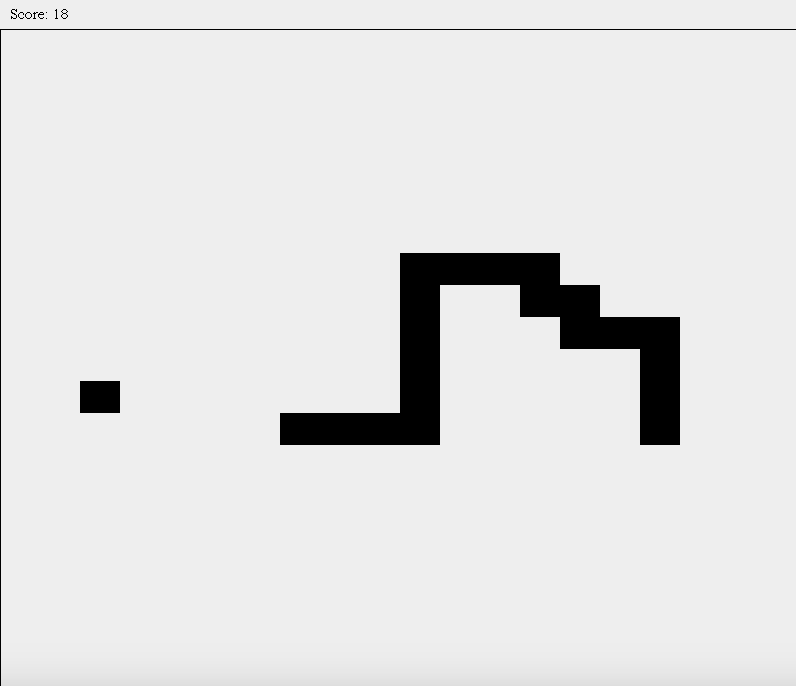
\includegraphics[width=0.4\textwidth]{SimpelSnake.png}}
	\hspace{0.1\textwidth}
	\subfloat[Advanced Snake]{\label{fig:advancedsnake}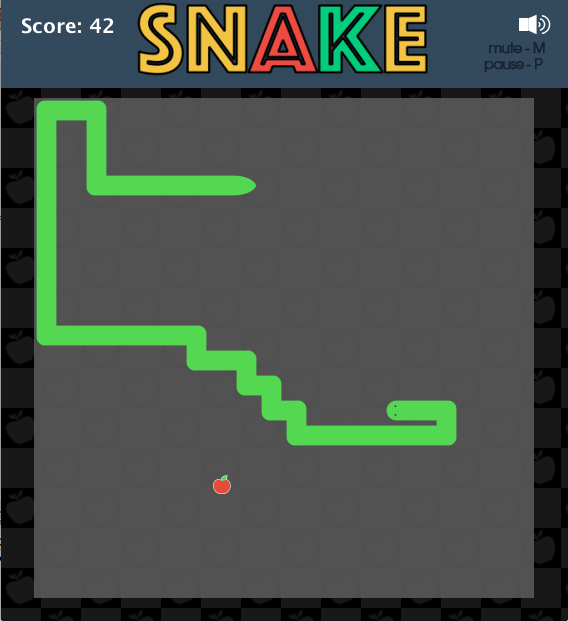
\includegraphics[width=0.32\textwidth]{snake2.png}}
	\caption{}
\end{figure}